\chapter{Proposed Scheme}\markright{Chapter 4: Proposed Scheme}\label{sec:proposed_scheme}

\section{idea}
Our goal is to design the defense scheme against each evasive technique on different targets, GSI and BD, to achive the practical CNN based IoT malware detection on IoT devices.
In order to accomplish our goal, we propose an evasion-resilient IoT malware detection scheme with invalidating adversarial byte sequences and 1D convolutional filters.  
The main idea of our scheme is that there still remain regions which contribute to decision making in both manipulated targets after the attacks.
We aim to improve the detection accuracy by statically extracting/enhancing each beneficial region of the target to the CNN model.

図 shows the manipulated area by adversaries and the area which have high degree of contribution for CNN to make decision on representative manipulated target.
The red area in each target is the area which has been manipulated.
In the case of AM, noise is added to the pixels, and in that of OM, the original BD is compressed or new code is inserted in these regions.
On the other hand, the yellow area is where contributes to decision making still remaining after the attack.
In the case of AM, it is the pixel region where noise cannot be added, and in that of OM, it is the byte sequence region which remain discretely after the compression.

In each defense scheme, the detection accuracy can be improved by feeding those yellow region effectively to the CNN model.
The representative schemes are explained in the following sections.



% The useful features which are applicable to encrypted data can be obtained by focusing on the untrusted destination servers since they are extracted without deep packet inspection.
Untrusted destination servers can be judged by identifying the level of SSL server certificates.  
% \We can obtain SSL server certificates of servers by using the Openssl command. 
The level of SSL server certificate is divided into three types, namely Extended Validation (EV), Organization Validation (OV) and Domain Validation (DV) certificates.
EV and OV certificates are highly trusted certificates, because passing the rigorous examination process such as certifying existence of organizations is required to acquire them. 
Meanwhile, since a DV certificate is an unreliable one due to lenient examination, the server which has a DV certificate is untrusted one.
In order to encrypt traffic data, attackers have to acquire SSL server certificates.
\We argue that attackers tend to exploit a DV certificate to encrypt malicious payload.
This is because it is hard for them to acquire EV and OV certificates due to rigorous examinations.
Furthermore, EV and OV certificates are expensive in comparison to a DV certificate.
Thus, attackers are not willing to introduce expensive certificates to their servers because the objective of them is earning money by selling sensitive information.
For the above reasons, in many cases, since attackers have no choice but to introduce a DV certificate to servers of them, their servers tend to be untrusted.
Hence, \our scheme can detect malwares by focusing on the communication with untrusted servers of attackers.

% In order to demonstrate \our argument, \we inspected the distribution of apps that communicate with DV servers.
% In order to demonstrate \our argument, \we inspected the percentage of communication with the server to which each SSL server certificate is introduced.
In order to demonstrate \our argument, \we inspected the percentage of apps communicating with DV servers.
As shown in \figurename~\ref{fig:ssl_inspection}, there exists the difference of the percentage of communication with DV servers between benign apps and malwares.
\begin{figure}[p]
	\centering
	\hspace{-55pt}
	% \includegraphics[scale=0.34]{./figure/dv_unknown_inspection.pdf}
	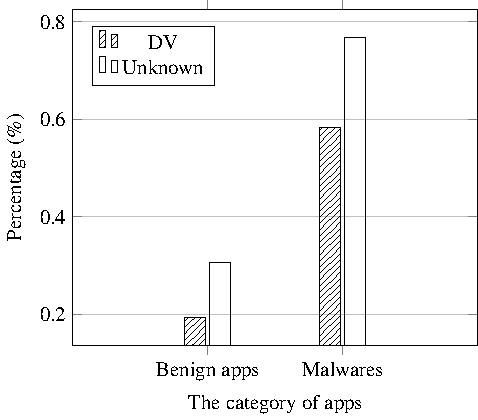
\includegraphics[scale=1.0, bb=9 9 200 200]{./figures/dv_unknown_inspection_tikz.pdf}
	% \includegraphics[scale=0.34]{./figure/ssl_inspection.pdf}
	\caption{The result of inspection regarding SSL server certificate} 
	\label{fig:ssl_inspection}
\end{figure}
\afterpage{\clearpage}
\newpage

Moreover, \we discovered the servers whose the level of certificates is unknown because of refusing access to the servers or timeout (hereinafter, such servers are called "unknown servers").
% \figurename~\label{fig:dist_unknown} shows the distribution of apps communicating with unknown servers.
As shown in \figurename~\ref{fig:ssl_inspection}, in comparison to benign apps, malwares tend to communicate with the unknown servers.
Thus, these results motivate us to extract SSL server certificate based features regarding DV and unknown servers.
\We can obtain the useful features which are hard to be disguised because attackers cannot easily introduce EV and OV certificates to the their servers.
Furthermore, \our features are applicable to encrypted data since they can be extracted without packet inspection.
We mainly extract two types of features from each traffic data of an app.
The first one is the total number of distinct IP address of untrusted servers, namely the DV and unknown servers because attackers tend to have several servers to evade detection.  
The second one is the feature based on the frequency of communication with DV and unknown servers.
As already mentioned in the Section \ref{sec:previous_scheme}, malwares tend to repeatedly try to communicate with untrusted servers of attackers compared with benign apps.
Hence, \we utilize the frequency of communication with untrusted servers for malwares detection.  

However, since benign apps also communicate with the untrussed servers, benign ones may be misjudged as malwares by using only SSL certificate based features.
In order to cope with such situation, \we focus on the fact that malwares inevitably have to require the permissions regarding malicious actions.
For example, malwares require a permission, READ\_PHONE\_STATE for obtaining device information.
By using such permission, malwares can send such data to untrusted servers of attackers.
Meanwhile, an app which does not have such permissions cannot send device information to external servers.
% Since malwares try to send such data to untrusted servers of attackers, there exists relation between the level of SSL certificates of destination servers and required permissions.
% Hence, required permissions are relevant to the level of SSL certificates of destination servers.  
Hence, in order to exactly express malicious features, \we introduce required permission based weight values to SSL certificate based features.
By doing this, \our scheme can reduce the misjudgement of the benign apps that communicate with untrusted servers.
Finally, SSL certificate based features to which weight values are assigned are used for detection by machine learning classifier.

\section{Algorithm}
In this subsection, \we explain the algorithm for extracting \our features.
The algorithm consists of four steps, namely network traffic collection, the level of SSL server certificate identification, SSL server certificate based feature generation and permission based weight assignment.

\subsection{Network Traffic Collection} 
Network traffic data of an app is captured in this step.  
In order to capture the network traffic data, \we execute an app on an Android emulator device provided by Android Studio \cite{studio2016official}.
\We execute a single app at one time on an emulator device to ensure that the exact network traffic data generated by each app is captured. 
% Accordingly, no app runs in the background when collecting traffic data of an app. 
\We then collect the network traffic packets of an app during the execution.
The traffic data are saved as PCAP format files by using tcpdump command \cite{jacobson1989tcpdump}.

\subsection{The Level of SSL Server Certificate identification} 
In this step, the level of SSL server certificate of each destination server is obtained to identify IP addresses of DV and unknown servers.
In order to confirm the level of SSL server certificate, IP addresses are extracted from PCAP format file by using T-shark command \cite{combs2017tshark}.  
\We then obtain a SSL server certificate of the server which corresponds to each IP address by using openssl command \cite{openssl}.  
In the EV and OV certificates, detailed geographic information of organizations is registered to certify the presence of organizations.
Meanwhile, a DV certificate does not include such information since it is the certificate which authenticates only the authority for using domain.
Thus, \we can judge whether each destination server is a DV server by focusing on the information registered in a certificate.  
Furthermore, a server can be regarded as an unknown server when refusing access to the server or timeout errors occur.
Accordingly, \we can identify IP addresses of both DV and unknown servers from among all destination servers by doing above procedures.

\subsection{SSL Server Certificate based Feature Generation}
SSL server certificate based features are calculated on the basis of IP addresses of DV and unknown servers.
\We calculate the frequency of communication with DV and unknown servers and the total number of distinct IP addresses of DV and unknown destination servers.
In terms of the frequency of communication, two types of the frequency are calculated by T-shark command.
The first one is the frequency of communication for sending packets to an app from DV servers.
The second one is the frequency of communication in the case where DV servers receive packets.
% These features are categorized as frequency based features.  
% The total number of distinct IP addresses of DV servers which communicate with an app is also calculated.
Similarly, same procedures are conducted for IP addresses of unknown servers.

\subsection{Permission based weight assignment}
In this step, permission based weight value is assigned to SSL server certificate based features.
First, \we have to calculate permission based weight values on the basis of the occurrence of permissions in the malicious train dataset in advance.
\We focus on only the dangerous permissions defined by the Android specification since these permissions are related to sensitive actions.
Let $\DANGEROUSPERMISSION = \{p_i|1\leq i \leq 24\}$ denote the set of dangerous permissions. 
% The dangerous permissions required by the apps in $\MALWARETRAIN$ are extracted for calculating weight value.
\We create $\MALWARETRAINPERMISSION$ which denotes the set of the malwares which request a dangerous permission $p_i$ in $\MALWARETRAIN$.
Here, $\MALWARETRAIN$ is the set of all malwares in the training dataset.
Then, \we create the set of the weight value for each permission $\WEIGHT = \{w_{p_i}|1\leq i \leq 24\}$.
A weight value $w_{p_i}$ for dangerous permission $p_i$ is calculated as the following equation:
\begin{equation}
  w_{p_i} = \frac{|\MALWARETRAINPERMISSION|}{|\MALWARETRAIN|}.  
\end{equation}
% Here, $\MALWARETRAINPERMISSION$ is the set of the malwares which request a permission $p_i$.

% For each app, the set of the all permissions required by each app $\APPPERMISSION = \{{p^{'}_j}|1\leq j \leq 300\}$ is created.
\We obtain $\APPPERMISSION$ that indicates the sets of the dangerous permissions required by each app . 
% , namely $\PERMISSIONINTER = \DANGEROUSPERMISSION \cap \APPPERMISSION$.
$\APPPERMISSION$ is represented as the following equation: 
\begin{equation} 
  \APPPERMISSION =
  \left\{
    \begin{array}{ll} 
      \{p_k|1\leq k \leq 24\} & (|\APPPERMISSION| > 0), \\
      \phi & (|\APPPERMISSION| = 0).
    \end{array}
  \right.
\end{equation}
After that, $w_{p_i}$ are assigned to SSL server certificate based feature $\FSSL$ of each app on the basis of $\APPPERMISSION$.
Accordingly, \our features are calculated as the following equation: 
\begin{equation} 
  f(\FSSL) = 
  \left\{
    \begin{array}{ll} 
      \FSSL * (1+ {\displaystyle \sum_{k=1}^{|\PERMISSIONINTER|}} w_{p_k})  & (|\PERMISSIONINTER| > 0), \\
      \FSSL & (|\PERMISSIONINTER| = 0).
    \end{array}
  \right.
\end{equation}

